\chapter{Two Stage Decoding of HMMs}\label{CHAPTER:TWOSTAGE}

In this chapter we will study several decoding techniques, which are aimed to
reduce systematic errors in sequence annotation.  We will illustrate our
approach using the HIV recombination prediction domain, discussed in Section
\ref{SECTION:HERD}. Here, the goal is to find out which parts of a recombinant
virus sequence originate in which subtype.  For this task, we have previously
developed the HERD decoding method \cite{Nanasi2010, Nanasi2010mgr} (Section
\ref{SECTION:HERD}) which performed better than the Viterbi algorithm. However,
in some cases the resulting annotation contains some systematic errors, for
example frequent switching between different subtypes. One such example can be
found in Figure \ref{FIGURE:HERD_BAD}. To mitigate such effects, one can use a
two-stage decoding strategy. First we search for the most probable footprint
$F$. The footprint is what is left from labeling after removing consecutive
identical labels. Formally it was defined in section
\ref{SECTION:DISTANTMEASURES} by definition \ref{DEFINITION::FOOTPRINT}. In the
second stage we find the annotation with footprint $F$ that maximizes the
expected reward or some other criterion. The second stage is forced to keep the
structure of footprint, and therefore rapid change of types as in Figure
\ref{FIGURE:HERD_BAD} is not possible (unless the footprint contains a large
number of recombinations).

More generally, in the first stage we search for the best guide, which is a
general constraint on the allowed annotation, for example in the form of
footprint or a set of labels. In the second stage, we find optimal annotation
using the selected guide. Example of such algorithm for the most probable ball
problem \cite{Brown2010, Truszkowski2011} discussed in Section
\ref{SECTION:DISTANTMEASURES}. In this this algorithm, two-stage were motivated
by the computational complexity, since optimizing the border shift distance is
NP-hard \cite{Brown2010}. Our motivation to use two-stage algorithm is to
improve their accuracy and decrease the amount of some systematic errors. 

In this chapter, we will focus mainly on the complexity of the first step:
finding the most probable guide. Complexity of the second step, namely finding
the annotation with highest expected gain without guides we studied in
\cite{Nanasi2010, Nanasi2010mgr}.  At first we give formal definition of the
two-stage algorithm. Then we show experiment illustrating effects of the
two-stage decoding on the HIV recombination detection problem. Further in this
chapter we prove that finding the most probable guide is for certain guide
functions NP-hard.


\begin{figure}
\begin{center}
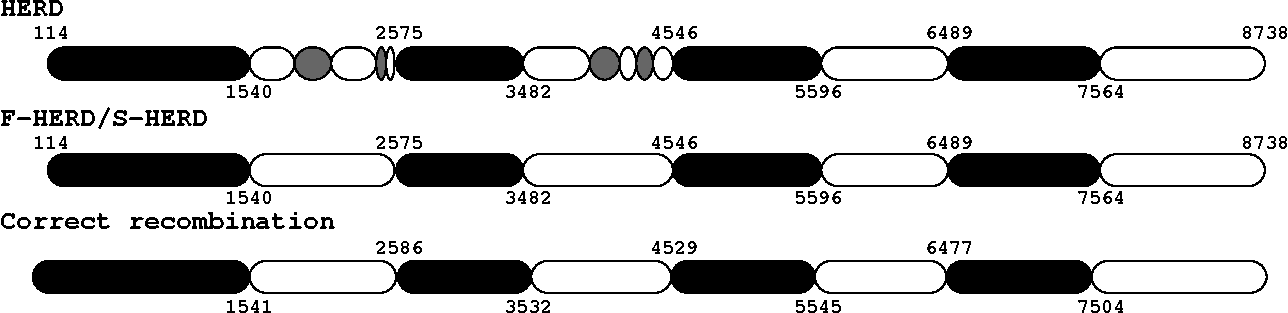
\includegraphics[width=14cm]{../figures/jcss/happyStory.pdf}
\end{center}
\caption[Example of annotation with systematic error.]{ 
Each row corresponds to one annotation of the same HIV recombinant, colors
represent virus subtypes. Unaltered HERD algorithm predicts a wrong
subtype and also contains too many segments. But restricting to the specified
footprint (F-HERD) or to the specified set (S-HERD) provides an almost correct
annotation without these errors.  }\label{FIGURE:HERD_BAD} 
\end{figure}

\section{Formal definition}
In this section we will define two-stage decoding algorithms, and the
generalization of the footprint function from the first stage, the guide
function. Additionally to the footprint, we define additional guide called
annotation set. Footprint was already defined in the definition
\ref{DEFINITION::FOOTPRINT}, and we denote the footprint of annotation
$\Lambda$ as $F(\Lambda)$. 

\begin{note}
The following definitions could also use state paths instead of 
annotations. However, annotations are more general, because by setting
$\lambda$ to the identity function, all annotations become state paths.
\end{note}

\begin{definition}[Annotation set]
Let $\pi = \pi_1\pi_2\dots \pi_n$ be a state path and $\lambda$ be coloring
function as in definition \ref{DEFINITION:ANNOTATION}.  The
\firstUseOf{Annotation set} of labeling $\Lambda$ is the set of labels visited
on the state path:
\[S(\pi) = \left\{\lambda(\pi_1), \lambda(\pi_2)\dots\lambda(\pi_n)\right\}\]
Annotation set of an annotation $\Lambda = \Lambda_1\Lambda_2\dots \Lambda_n$
is the set
\[S(\Lambda) =
\left\{\Lambda_1,\Lambda_2,\dots\Lambda_n\right\}\]
A \firstUseOf{state set} is an annotation set when the labeling function is the
identity function.\label{DEFINITION:ANNOTATION_SET}
\end{definition}

Two-stage decoding system can be described in Highest Expected Gain framework
introduced in section \ref{SECTION:HEG}. At first, we define guide and guide
function.

\begin{definition}[Guide function, guide relation, guide]
Let $H$ be an HMM, and $f$ be an annotation gain function. Let $L$ be the set of
all annotations, $W$ be an arbitrary set. We call any function
$R:L\to W$ a \firstUseOf{guide function} and $R(\Lambda)$ is the
\firstUseOf{guide} of annotation $\Lambda$.

A \firstUseOf{guide relation} is a relation $\hat{R}\subseteq L\times W$
with the property that for all $\Lambda\in L$, $(\Lambda, R(\Lambda))\in \hat{R}$.

We will define the probability of guide $r$ given sequence $X$:

\begin{equation}
\prob{r\mid X, H} = \sum_{\Lambda \in L, R(\Lambda)=r} \prob{\Lambda\mid X, H}
\end{equation}

\end{definition}

A natural way of defining guide relation is the following: $(\Lambda, r)\in
\hat{R}$ if and only if $R(\Lambda)=R$. However, in some cases it might be
useful to relax the restriction provided by the guide. 

Note that we can see a guide as a generalization of an annotation. However, our
use of guides is quite different from our use of annotations. While annotations
are the final product, purpose of guides is to capture some important
properties of the input, that can be subsequently used to find the correct
annotation. Finally, we can formally define the two-stage decoding:

\begin{definition}[Two-stage decoding]
Let $H$ be an HMM, $f$ be an annotation gain function, $R$ be a guide 
function and $W$ be a set of all possible guides. Let $X$ be a sequence of
interest and $L$ be the set of all annotations of $X$. In the \firstUseOf{two-stage
decoding} we search for annotation $\Lambda$, defined as:

\begin{equation}
\Lambda = \arg\max_{\Lambda'\in L, (\Lambda', r)\in \hat{R}}E_{\Lambda_X\mid
X,H}[f(\Lambda_X,\Lambda')]\label{EQUATION:HIGHEST_EXPECTED_RESTRICTED_REWARD}
\end{equation}
where guide $r$ is defined as
\begin{equation}
r = \arg\max_{r'\in W}\prob{r'\mid H, X}
\label{EQUATION:MOST_PROBABLE_RESTRICTION}
\end{equation}
\end{definition}

Finding the most probable guide can be decoupled from finding the
annotation with highest expected reward. Implementing search with guides is straightforward, and we will
discuss it later.

Note that we could use a different method to select guide $r$. While it is
possible to use gain functions for defining optimization criteria to select
guide (and altering the equation \ref{EQUATION:MOST_PROBABLE_RESTRICTION}), 
we did not study such variations.

\section{Experiments}

In this section we apply the two-stage decoding methods on the HIV
recombination detection problem. Our goal is to illustrate the effect and
usefulness of the two-stage decoding algorithms, not to compare it with the
other methods for recombination detection.  We will describe the HIV
recombination detection domain, two two-stage decoding algorithm and show
experiment on the artificial dataset of recombinant HIV sequences.

In section \ref{SECTION:HERD} we described HERD decoding. It was used with
jumping HMMs \cite{Schultz2006} for detecting recombinations in HIV virus.
However, using this criteria lead to two artefacts: 
\begin{itemize}[itemsep=-1mm]
\item Producing annotations with many short recombinations.  
\item Producing recombinations of wrong virus subtype.  
\end{itemize}
Example of both type of
errors are illustrated in Figure \ref{FIGURE:HERD_BAD}.

\subsection{Application Domain}
We use the problem of recombination detection in HIV virus for the demonstration of
usefulness of two-stage decoding.  This section contains background information
about data used in the experiment.

\begin{figure}
\begin{center}
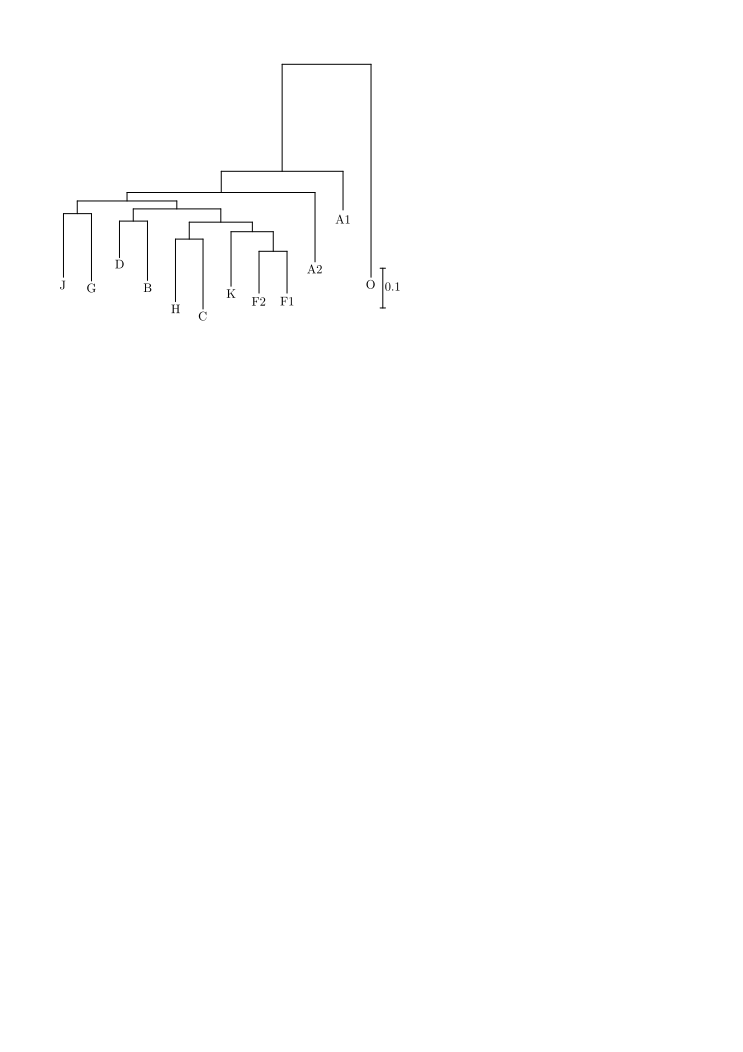
\includegraphics{../figures/hiv_M1strom}
\end{center}
\caption[Phylogenetic tree of the HIV-M1 group]{Phylogenetic tree of the HIV-M1
group of genomes with outgroup sequences from the of HIV-O group generated by phyml \cite{Guidon2003}
from the database distributed with jpHMM \cite{Schultz2006}. Figure was originally
used in \cite{Nanasi2010mgr}. The lengths of the branches correspond to 
evolution distances.  }\label{app:figure:phil}
\end{figure}

The genome of the HIV virus is an RNA sequence roughly $9000$ bases long.
Mutation rate of the HIV virus is high \cite{Schultz2006}, and additionally HIV virus is
categorized into several \firstUseOf{subtypes} \cite{Robertson2000} based on sequence
similarity. Phylogenetic tree of subtypes is show in figure
\ref{app:figure:phil}.  Subtypes A and F are further divided into
\firstUseOf{sub-subtypes} A1, A2 and F1, F2.  Due to high sequence similarity,
subtypes B and D are sometimes recognized as sub-subtypes of subtype BD
\cite{Robertson2000}.

Additionally to high mutation rate, \firstUseOf{recombination} occurs in
evolution of HIV virus \cite{Robertson2000}. Recombination of two source viruses $v_1$
and $v_2$ is a mosaic virus which contains parts from both $v_1$ and $v_2$.  The
relative position of individual parts is retained, so each region of the
recombinant virus originates from the corresponding region in the source virus.
There can be multiple recombination points within the same virus, and since
recombination can occur between two recombinants, there can be multiple source
subtypes or sub-subtypes in one recombinant. 

Given a recombinant sequence $X$, the goal of recombination detection is to
label each base $x$ of sequence $X$ with the subtype from which $x$ originates.
The input sequence does not have to contain recombination. In such case the
annotation of the sequence contain only single subtype. The set of annotation
symbols therefore contains all subtypes/sub-subtypes of the HIV virus. 

\subsection{Model}
\label{HERD:METHODS}
In our experiments, we use \abbreviation{jumping HMM}{jpHMM}  developed for
recombination detection  by {\it Schultz et al. (2006)}. The main building
block of the jpHMM are profile Hidden Markov Models (profile HMMs).

\begin{figure}
\begin{center}
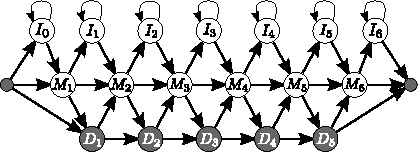
\includegraphics[width=10cm]{../figures/profile_hmm}
\end{center}
\caption[Profile HMM]{Example of a profile HMM of length $6$. Shaded states are
silent. The leftmost shaded state is the init state, the rightmost
shaded state is the final state. Figure is from \cite{Nanasi2010mgr}.}\label{FIGURE:PROFILEHMM}
\end{figure}

Profile HMMs are HMMs with a special topology used for matching certain
motifs \cite{Durbin1998}. Profile HMM of length $n$ consists of match states
$M_1,M_2,\dots, M_n$, insert states $I_0, I_1, \dots, I_n$, silent delete states
$D_1, D_2,\dots, D_n$ and silent init state and silent final state. All states are
connected by transitions as in the figure \ref{FIGURE:PROFILEHMM}. A motif is
represented by the chain of match states, each with its own emission distribution.
Insert states model (short) insertions between positions of the motif. Delete states allow to
skip some parts of the motif. A profile HMM can be obtained from an alignment of
similar sequences; match states then represent columns of the alignment.
Not all of the columns correspond to match states; columns that
contains gaps above some threshold are usually omitted \cite{Durbin1998}. 

Jumping HMMs are built upon profile HMMs \cite{Schultz2006}. We start with an
alignment of all HIV sequences and construct a profile HMM for each subtype or
sub-subtype (it depends on whether we want to distinguish between
sub-subtypes).  We then add global init state and global final state to connect
profiles in parallel.  Column numbers of each match, insert, and delete states
are preserved, so we know the corresponding column for all submodels.
Transitions between different profiles are added to model recombinations: These
"jump" transitions always end in the state that corresponds to the nearest
column of the original alignment following their source column. Jump from
column $c_1$ in subtype $A$ to column $c_2>c_1$ in subtype $B$ is allowed if
and only if there are no states in the profiles of $A$ or $B$ corresponding to columns
between $c_1$ and $c_2$. A simplified topology of a jpHMM is in figure
\ref{app:fig:jpHMM}. More details can be found in \cite{Schultz2006}.

\begin{figure}
\begin{center}
\includegraphics[width=10cm]{../figures/jumping_hmm}
\end{center}
\caption[Jumping HMM]{The simplified structure of a jpHMM. Insert and delete states
are omitted from the figure for readability. Picture is taken from our previous
work \cite{Nanasi2010mgr}}\label{app:fig:jpHMM}
\end{figure}

\subsection{Algorithms}

In this section we describe the HERD algorithm and how to modify the Viterbi
algorithm and the HERD to use footprint and the annotation set as the guides.
We denote HERD's gain function, described in section \ref{SECTION:HERD}, as
$f_{HERD}$ (note that the gain function of the Viterbi algorithm is $f_V$).
Details of the algorithm that optimizes this gain function can be found in
\cite{Nanasi2010, Nanasi2010mgr}. We use the footprint and the annotation set
as a guide functions. In case of footprint, we use the natural way to define
guide relation, however in case of the annotation set we use guide relation
$\hat{R}_S$ defined as follows: \[(\Lambda, r)\in \hat{R}_S\Leftrightarrow
R(\Lambda)\subseteq r\] The reason for using this guide relation is that it
allows us to use simpler and faster optimization algorithm. This is not a
problem because HERD have problem with detecting additional wrong subtypes, not
missing the correct one.  In our tests it never occurs that the resulting
annotation had different set than the most probable set from the first stage of
the algorithm.  In the following text, we will use the term
\firstUseOf{segment}, which is the maximal single-colored consecutive
subsequence of annotation.

The original HERD algorithm can be decomposed into two phases. In the first
phase, it constructs an \firstUseOf{annotation graph}.  An annotation graph is
a graph in which each path from the start vertex to the end vertex represents
an annotation. The length of such a path equals to the expected gain of the
corresponding annotation. The longest path in the annotation graph therefore
corresponds to the annotation with the highest expected gain. Annotation graph
is directed and acyclic and its structure is described in Figure
\ref{HERD:figure:annotation_graph}. In the second phase we find the longest
path in this graph and convert it to the annotation. Since the annotation graph
is directed and acyclic, it is possible to find such a path in polynomial time
\cite{Nanasi2010mgr}.

To add guides, we need to change the second phase of the algorithm. We will be
searching for an annotation restricted to the guide with the highest expected
gain. If the guide function is an annotation set,  we simply remove vertices with
colors that are not in annotation set from the annotation graph and use the original
algorithm described in \cite{Nanasi2010mgr}. Since trimming the annotation graph
can be done trivially in linear time, this does not change the computational
complexity of the HERD algorithm.

\begin{figure}
\begin{center}
\includegraphics{../figures/herd_graph}
\end{center} 
\caption[Annotation graph]{Part of a path in an annotation graph with the
corresponding annotation. A node with color $c$ and caption $(b,w)$ represents
the vertex $(b,c,w)$ of the graph. The dashed lines connect each vertex to its
corresponding segment. $(b, c, w)$ corresponds to the beginning of $c$-colored
annotation segment starting at position $b$. End of the segment is determined
by the following vertex in the path; therefore each edge in the graph
corresponds to a possible annotation segment. The length of an edge is the
expected gain of the corresponding annotation segment. If $w$ is less than
maximal window width $W$, which is a parameter of the HERD algorithm, the edges
from such vertex are allowed only to vertices of the form $(b+w, *, *)$ where
$*$ can be any valid value. If $w=W$, then outgoing edges are of the form
$(b+W+k, *, *)$ where $k\leq0$.  Figure is from our previous work
\cite{Nanasi2010mgr}}\label{HERD:figure:annotation_graph} 
\end{figure}

Using the footprint as a guide requires more changes to the algorithm then just
removing vertices with colors that are not in the footprint; we also alter the
dynamic programming formula for computing the longest path.  We order vertices
of the annotation graph topologically from start to end vertex into sequence
$v_0, v_2, \dots v_{n-1}$ where $n$ is the number of vertices in the annotation
graph, $v_0$ is the init vertex and $v_{n-1}$ is the end vertex.  This will be
the order in which the dynamic programming equations will be computed.  Let
$f=f_0f_2\dots f_{k-1}$ be the footprint we use as a guide and $V[i, j]$ be the
length of the longest path ending in $v_i$ that has footprint $f[:j]$.
Therefore the length of the longest path with footprint $f$ is $V[n - 1, k]$.
If $E$ is the set of all edges and $C(v_i, v_j)$ is the weight of an edge
$(v_i, v_j)$, then $V[i, j]$ can be computed by following equations: 
\begin{align} 
V[0, 0] &= 0 \\ V[0, j] &= -\infty, 0< j \leq k \\
V[i, j] &= \max_{i', (v_{i'}, v_i)\in E} 
\begin{cases} 
C(v_i', v_i) + V[i', j]& \text{if $\lambda(v_i) = \lambda(v_{i'})$}\\
C(v_i', v_i) + V[i', j-1]& \text{if $\lambda(v_i) \not= \lambda(v_{i'})$ and $\lambda(v_{i'})=f_{j-1}$}\\
0 & \text{otherwise} 
\end{cases} 
\end{align}

Note that since we have ordered vertices topologically, to compute $V[i, j]$ we
use only values of $V[i', j']$ where $i'< i, j'\leq j$. Therefore we can compute
$V$ in increasing order of $i$. The longest path can be computed using
back-tracing as in section \ref{SECTION:NEEDLE}. The time and memory complexity 
of this part of the algorithm increased by the factor of $k$. Therefore the
time complexity increases to $O(mWC|E|+mkC^2W^2)$ where $C$ is the number of
colors (labels), $W$ is the window size, $m$ is the length of the sequence and
$|E|$ is the number of transitions in the HMM.  Space requirements increased to
$O(\sqrt{m}Cn+WCnk+mkC^2)$. However, in practice guide contains only a small
number of colors and as a result, graph is much smaller then in the unguided
version. Implementation details of other parts of an algorithm can be found in
\cite{Nanasi2010mgr}.

As we will show in this chapter, finding the most probable set or the most
probable footprint are NP-hard problems.  Therefore we used heuristic algorithm
implemented in the from program balls \cite{Brown2010}, which is also described
in section \ref{SECTION:DISTANTMEASURES}. Note that the balls algorithm
estimates the footprint by sampling state paths and selecting the most
frequent footprint of sampled paths. For using the set as a guide, we have chosen
the set of labels used in the footprint guide, since these sets were almost
always correct. 

Altering the Viterbi algorithm to use set as an restriction is as simple as for
the HERD; we only need to to ignore states that are not in the guide set. We
can do it by removing state that are not in the guide set from the HMM without
normalizing the transition probabilities. 

For optimizing the Viterbi algorithm with footprint $f$ as an guide can be done
by computing following equations:
\begin{align}
V[0,v, 0] &= I_{v}e_{v,X_0}, \lambda(v) = f_0\\
V[0,v, 0] &= 0, \lambda(v) \not= f_0\\
V[0,v, l] &= 0, l>0  \\
V[i,v, l] &= \max_{u\in V}\begin{cases}
V[i-1,u, l]a_{u,v}e_{v,X_i}& 
\text{if $\lambda(v) =\lambda(u)$}\\
V[i-1,u, l - 1]a_{u,v}e_{v,X_i} &
\text{if $\lambda(u) = f_{l-1}$ and $\lambda(v) = f_{l}$}\\
0 & \text{otherwise}
\end{cases}\\
\end{align}
where $v\in V,0<i<n$. Computation of back-links $B[i, v, l]$ are analogous to
the computation of $V[i, v, l]$ as in the Viterbi algorithm. Note that these
equations are the original Viterbi equations from Section \ref{SECTION:VITERBI}
with additional dimension: the position $l$ in the footprint. The time
complexity of this algorithm is $O(nm^2k)$, where $k$ is the length of the
footprint. This algorithm is $k$ times slower than the Viterbi algorithm.

\subsection{Data and results}
We created an artificial dataset of recombinant HIV sequences and run HERD and
the Viterbi algorithm (VA) with two guide functions: annotation set and
footprint. HERD was run with default parameters, $\gamma=0.2, W=10$. The model
was trained using jpHMM program on the alignment of HIV sequences distributed
with jpHMM \cite{Schultz2006}. We removed $10\%$ of sequences from this
alignment before training data and used them for evaluation. We refer to the
alignment distributed with jpHMM as the \firstUseOf{source alignment}.

Artificial testing sequences were generated by alternating segments of two real
sequences from different subtypes.  These alternating segments were selected
from an alignment of original sequences. We did experiments with two types of
segment lengths: either $200-300$ (short) or $950-1050$ (long) with additional
$0-750$ and $0-500$ bases for the first and for the last segment respectively.
The Length of each segment was drawn from the uniform distribution.

Apart from two different recombination length, we also evaluated algorithm of
recombinants of sequences from same subtypes but different sub-subtypes, which
gave us $4$ different data sets. For all datasets we generated $150$
recombinants of two sequences. For subtypes we use subtypes A, BD, C, F, G. For
sub-subtypes we have used sub-subtype pairs A1-A2, B-D and F1-F2. \todo{Tieto
experimenty by som radsej zbehol este raz}

To measure accuracy of the algorithms and amount of systematic errors, we use
the following metrics.
\begin{enumerate}[itemsep=-1mm]
\item {\bf \%id}: Percentage of the bases with correctly predicted label.

\item {\bf Segment specificity}: Percentage of the number of correctly predicted
segments out of the number of all predicted segments. Segment is correctly
predicted if its boundaries are within $10$ bases of the correct boundaries.

\item {\bf Segment sensitivity}: Percentage of the number of correctly predicted
segments out of the number of segments in the correct annotation.

\item {\bf \%correct footprints}: Percentage of correctly predicted footprints.

\item {\bf Footprint distance}: Edit distance of predicted footprint and
correct footprint normalized by the length of the correct footprint
(averaged over all samples).

\item {\bf Set specificity}: Percentage of the number of correctly predicted label
types out of the total size of predicted label set.

\item {\bf Set sensitivity}: Percentage of the number of correctly predicted label
types out of the total size of correct label set.

\end{enumerate} 
Aim of measures $1-3$ is to quantify the performance of the algorithm in terms
of ability to correctly predict the correct annotation. Measures $4-7$ quantify
the amount of previously mentioned systematic errors in the predicted annotation.

We use three versions of HERD and VA in our experiments: original algorithm,
version with annotation set as a guide denoted by S-HERD (S-Viterbi) and
version using footprint as a guide denoted by F-HERD (F-Viterbi). The results
of experiments are in the table \ref{HERD:EXPTABLE}. 

\begin{table*}
\begin{center}
\begin{tabular}{cccccccc}
&{\bf \%id}&\bf segment&\bf segment&\bf \%correct&\bf footprint&\bf set&\bf  set\\ 
&&\bf sp.& \bf sn.& \bf footprints&\bf distance&\bf    sp.&\bf  sn.\\ 
\hline
\hline
\multicolumn{8}{l}{\bf subtypes, short recombination length}\\\hline
HERD     &88.09     & 65.59     &\bf 67.71  & 30.67     &     0.0728    & 56.67      &\bf 100.0  \\
S-HERD   &\bf 88.55 & \bf 68.17 &\bf 67.71  & \bf 37.33 & \bf 0.0699    & \bf 99.33  &\bf 100.0  \\
F-HERD   &84.71     & 65.02     & 58.19     & 2.67      &     0.1653    & \bf 99.33  &\bf 100.0  \\\hline
Viterbi  &     86.33&     62.73 &    61.31  &     19.33 &     0.1097    &     68.67 &\bf 100.0  \\
S-Viterbi& \bf 87.01&\bf  64.33 &\bf 62.12  &  \bf 26.0 & \bf 0.100.08    & \bf 99.33 &\bf 100.0  \\
F-Viterbi&     84.75&     61.99 &    55.57  &      2.67 &     0.1653    & \bf 99.33 &\bf 100.0  \\\hline\hline
\multicolumn{8}{l}{\bf sub-subtypes, short recombination length}\\\hline
HERD     &\bf 72.72 & 32.79     & \bf 27.56 & \bf 0.0   & \bf 0.3416    & 19.33     &\bf 100.0  \\
S-HERD   &72.33     &\bf 35.77  & 26.59     & \bf 0.0   &     0.3937    & \bf 100.0   &\bf 100.0  \\
F-HERD   &68.05     &30.65      & 16.97     & \bf 0.0   &     0.4777    & \bf 100.0   &\bf 100.0  \\\hline
Viterbi  &     69.34&     30.54 &     21.04 & \bf   0.0 &     0.4729    &      32.0 & 99.33   \\
S-Viterbi&\bf  70.21& \bf 32.28 & \bf 21.37 & \bf  0.0  & \bf 0.4715    & \bf 100.0   & 99.33   \\
F-Viterbi&     67.91&     26.18 &     14.67 & \bf  0.0  &     0.4777    & \bf 100.0   & \bf 100.0 \\\hline\hline
\multicolumn{8}{l}{\bf subtypes, long recombination length}\\\hline
HERD     &93.86     & 50.20     & 61.82     & 76.67     &     0.0579    & 77.33     &\bf 100.0  \\
S-HERD   &94.12     & 53.46     & 63.68     & 98.67     &     0.0030    &   \bf 100.0 &\bf 100.0  \\
F-HERD   &\bf 94.19 & \bf 53.57 & \bf 63.83 & \bf 100.0   & \bf    0.0    & \bf 100.0   &\bf 100.0  \\\hline
Viterbi  &     93.82&     49.09 &     59.40 &     86.67 &     0.0230    &     86.67 &\bf 100.0  \\
S-Viterbi&     93.96&     50.24 &     60.10 &      98.0 &     0.0046    & \bf 100.0.0 &\bf 100.0  \\
F-Viterbi& \bf 93.99& \bf 50.61 & \bf 60.33 & \bf 100.0 & \bf    0.0    & \bf 100.0.0 &\bf 100.0  \\\hline\hline
\multicolumn{8}{l}{\bf sub-subtypes, long recombination length}\\\hline
HERD     &84.10     & 19.87     & 25.63     & 21.33     &     0.4089    & 29.33     &\bf 100.0  \\
S-HERD   &83.90     & 24.87     & 28.55     & 47.97     &     0.1026    &     98.65 &\bf 100.0  \\
F-HERD   &\bf 85.03 & \bf 26.65 & \bf 30.24 & \bf 98.0  & \bf 0.0038    & \bf 98.67 &\bf 100.0  \\\hline
Viterbi  &     84.75&     22.46 &     26.18 &    40.0   &     0.1520    &     56.67 &\bf 100.0  \\
S-Viterbi&     85.23&\bf  24.61 & \bf 27.70 &    64.0   &     0.0654    & \bf 98.67 &\bf 100.0  \\
F-Viterbi&\bf  85.39&     24.57 & \bf 27.70 &\bf 98.0   & \bf 0.0038    & \bf 98.67 &\bf 100.0  \\
\end{tabular}
\end{center}
\caption[Accuracy of decodings with fixed footprint/set.]{Results of experiments
on four data sets. Note that larger values are better for all columns  except
{\it footprint distance} column where a lower value is better. The best value out of
each column is shown in bold.}\label{HERD:EXPTABLE}
\end{table*}

In general, we expect short recombination length to be harder than long
recombination length and distinguishing between sub-subtypes to be harder than
distinguishing between subtypes. Both of these expectations were observed in
the results. In all experiments on recombinants with long recombination length,
footprint algorithms outperformed their non-guided versions in all metrics,
especially with the metrics $4-7$: for HERD, the fraction of correct footprint
was increased from $76.67\%$ to $100\%$ in case of subtypes and from $21.33\%$
to $98\%$ in case of sub-subtypes (similarly for VA). However on recombinants
with short recombination length, used footprints were wrong most of the time
and in the sub-subtypes dataset all of the algorithms predict zero correct
footprints.  In fact, accuracy of F-HERD and F-Viterbi decreased in all metrics
except for annotation set specificity and sensitivity. This and increase in
footprint distance suggest the problem might be cause by heuristic methods for
finding the best footprint and that improvements in these methods are needed;
to check this, we computed the probability of predicted and correct footprints.
For short recombination length and sub-subtypes, $88.67\%$ of predicted
footprints have lower probability than the correct footprint, $2.67\%$ have the
same probability and $8.67\%$ have higher probability than the correct
footprint.  For the same recombination length and subtypes, $60.67\%$ of the
predicted footprints have lower probability and $39.33\%$ have higher
probability than the correct footprint.  For the long recombination lengths,
footprints which were not correctly predicted have higher probability than the
correct footprint.

Methods with set as an guide performs slightly worse than footprint based
methods on the data sets with long recombination lengths, but the metrics were
still significantly better than unguided HERD algorithm.  Additionally, using
set as an guide for short recombination length was not performing worse than
original algorithm; accuracy was similar.

\section{Computational complexity problems}

In the previous experiments, we demonstrated that the two-stage algorithm can
be a useful technique to improve HMM decoding algorithm. In this and following
sections we will discuss theoretical aspects of defining guides and finding the
most probable guides. In particular, we show that the following problems are
NP-hard: \firstUseOf{the most probable set}, \firstUseOf{the most probable
footprint}, and \firstUseOf{the most probable restriction}. The last problem is
variant of the most probable set. In this section we define these problems and
state the main results. The following sections then discuss individual problems
and prove the results.

\begin{definition}[The most probable set problem] Given an HMM $H$, sequence $X$ of
length $n$ and a number $p\in [0,1]$, decide if there exists a set of states $S$
such that $\prob{S(\pi) = S, X\mid H} \geq p$.
\end{definition}

\begin{theorem}
The most probable set problem is NP-hard. \label{THEOREM::NPSET}
\end{theorem}

In the most probable set problem, we consider only paths that use all
of the states from the annotation set. As in the experiments, it is more natural to 
include also paths that use only a subsets of annotation set. Therefore we
might be interested in maximizing 
\[
\prob{S(\pi) \subseteq S, X\mid H} = \sum_{\pi'\subseteq\pi}\prob{S(\pi') = S, X\mid H}
\]
However, this probability is trivially maximized by the set of all labels. To
get a meaningful problem definition, we can restrict the size of the annotation
set to be $l$:

\begin{definition}[The most probable restriction problem]
Given an HMM $H$, sequence $X$, integer $l$ and number $p\in[0,1]$, decide if
there exists a subset of states $S$ of size $l$, such that
$\prob{S(\pi)\subseteq S, X\mid H} \geq p$.
\end{definition}

\begin{theorem}
The most probable restriction problem is NP-complete. \label{THEOREM::NPREST}
\end{theorem}

Finally, we also show that the most probable footprint problem is NP-complete.
\begin{definition}[The most probable footprint problem]
Given an HMM $H$, sequence $X$
of length $n$ and a number $p\in [0,1]$, decide if there exists a footprint $F$
such that $\prob{f(\pi) = F, X\mid H}\geq p$.
\end{definition}

\begin{theorem}
The most probable footprint problem is NP-complete even if a labeling function is the identity function.
\label{THEOREM::NPFOOT}
\end{theorem}
Note that if we allow labeling function to be arbitrary, we can reduce the most
probable annotation problem to the most probable footprint problem, we only
need to make sure that it is not possible to have two consecutive states with
same label in possible state path. It can be done by adding states with new
label in the middle of the transitions, that generates new symbol and adding
such symbols between symbols of the input sequence. In such case, the most
probable annotation and the most probable footprint will be identical.

First we show combinatorial proof of theorem \ref{THEOREM::NPSET}. Then we show
proof of theorem \ref{THEOREM::NPREST}. Finally we show proof of theorem
\ref{THEOREM::NPFOOT} by showing $8$-state HMM for which is NP hard to find the
most probable footprint and then we extend this proof to theorem
prove theorems \ref{THEOREM::NPSET} and \ref{THEOREM::NPREST}.

\section{The Most Probable Set Problem}
\label{sec:set}

%\begin{definition*}[The most probable set problem] Given an HMM $H$, sequence $X$ of
%length $n$ and a number $p\in [0,1]$, decide if there exists a set of states $S$
%such that $\prob{S(\pi) = S, X\mid H} \geq p$.
%\end{definition*}

In this section, we prove NP-hardness of the most probable set problem, theorem
\ref{THEOREM::NPSET}.

We will use a reduction from the maximum clique
problem \cite{Garey1990}.  Given a graph $G=(V,E)$ and a clique
size $k$, we first choose a suitable threshold $k'\ge k$, as
detailed below, and construct a graph $G'=(V',E')$ such that $G'$ has
a clique of size $k'$ if and only if $G$ has a clique of size
$k$. This is achieved simply by adding $k'-k$ new vertices and
connecting each of the new vertices to all other vertices in $V'$.
As long as $k'-k$ is not too large, this transformation can be done in
polynomial time.

In the next step, we use $G'$ and $k'$ to construct an HMM $H_{G'}$, an input
sequence and a probability threshold. Every state set in $H_{G'}$ with
probability above threshold for the given sequence corresponds to a clique of
size $k'$ in graph $G'$. We will use the following straightforward way of
converting a graph to an HMM.

\begin{definition}\label{GraphHMM}
Let $G=(V,E)$ be an undirected graph (without self-loops). 
Then the \emph{graph HMM} $H_G$ is defined as follows:
\begin{itemize}[itemsep=-1mm]
\item Its set of states is $V\cup \{\psi\}$, where $\psi\notin V$ is a
  new state called the error state.
\item Its emission alphabet is $\{0,1\}$.
\item Each state $v\in V$ has initial probability $I_{v} = 1/|V|$, the
error state has initial probability $I_{\psi}=0$.
\item Each state $v\in V$ emits 0 with probability 1, the error state emits 1 
with probability 1.
\item Transitions with non-zero probability between states $u,v\in V$
  correspond to edges in $E$:
$$a_{u,v}=\begin{cases}
\frac1{|V|} & \{u,v\}\in E\\
0 & \text{otherwise}
\end{cases}$$
\item $a_{u,\psi}=1-\sum_{v\in V}a_{u,v}$
and $a_{\psi,u}=0$ for all $u\in V$. The error state has a self-transition with
probability 1: $a_{\psi,\psi}=1$.
\end{itemize}
\end{definition}

The purpose of error state $\psi$ is to level the probabilities of admissible
state paths without $\psi$ to the same probability. Since $\psi$ is the only
state that generates $1$, only sequences of form $X=0^n$ can be generated by
admissible state paths without the error state. Emission probabilities on such
strings are $1$, initial probability and all transitions are equal to
$|V|^{-1}$, and therefore $\prob{\pi, X=0^n\mid H_G,n} = |V|^{-n}$.  Each such
path corresponds to walk in graph $G$. Each set of states in $H_G$ naturally
corresponds to a subset of vertices. The probability of the set is proportional
to the number of corresponding walks in the graph $G$. Therefore we will count
the number of special walks in induced subgraphs of $G$.

\begin{definition}
Let $G=(V, E)$ be a graph and $S\subseteq V$ be an arbitrary set of its
vertices.  Then walk $w=v_1v_2\dots v_n, (v_i\in V)$ of length $n-1$
\firstUseOf{covers} set $S$, if and only if $\left\{v_1, v_2, \dots, v_n\mid
1\leq i\leq n\right\}=S$.  We say that walk $w$ covers graph $G$ if $w$ covers
the whole set of vertices $V$.

\end{definition}
In other words, a walk covers set $S$ if it uses only vertices from $S$ and each
vertex from $S$ is used at least once.

Let $Y(n, G)$ be the number of graph covering walks of length $n-1$. Since a walk
of length $n - 1$ contains $n$ vertices, $Y(n, G)=0$ if $n<|V|$. We consider a
special case of this formula for complete graphs: Let $K_k$ be
complete graph with $k$ vertices, then $D(n, k) = Y(n, K_k)$. The following claim
clearly holds:

\begin{lemma}\label{NotCliqueIsSmaller}
If $G$ is a graph with $k$ vertices and $n\ge k$, then
$Y(n,G)\le D(n,k)$ with equality only for $G=K_k$. 
\end{lemma}

In our reduction, we use HMM $H=H_{G'}$ and $X=0^n$ for a suitable choice of
$n$ and $k'$ discussed below. We will set threshold $p$ to $D(n,k')/|V|^{n}$.
Clearly, if the input graph $G$ has a clique $S$ of size $k$, graph $G'$ has a
clique $S'$ of size $k'$ and there are $D(n,k')$ walks of length $n-1$ that cover
$S'$. Each such walk corresponds to one state path, and therefore the
probability of the set of states $S'$ is exactly $p$. 

In order to prove the opposite implication "if there exists a set of states with
probability $p$ then there is clique of size $k$ in $G$", we need suitable choices
of $n$ and $k'$. Table \ref{DNKTable} shows values of $D(n,k)$ for
small values of $n$ and $k$. For a fixed length of walk $n$, the
number of walks in $K_k$ initially grows with increasing $k$, as we
have more choices which vertex to use next, but as $k$ approaches $n$,
$D(n,k)$  may start to decrease, because the walks are more constrained by
the requirement to cover every vertex. We are particularly interested in
the value of $k$ where $D(n,k)$ achieves the maximum value for a fixed $n$. 
In particular we use the following notation:
$$M_{n} = \min\left\{k ; D(n,k) = \max_{0\leq k'\leq
  n}D(n,k')\right\}$$
  
Note that if there are multiple values
of $k$ achieving maximum, we take the smallest one as $M_n$.  In our
reduction, we would like to set $n$ to be the smallest value such that
$M_n=k$, but we were not able to prove that such $n$ exists for each $k$.
Therefore we choose as $n$ the smallest value such that $M_n\ge k$, and 
we denote this value $n_k$. As $k'$ we then use $M_{n_k}$. The following 
lemma states important properties of $n_k$ and $M_{n_k}$. 

\begin{table*}
\begin{center}
\begin{tabular}{|c||c|c|c|c|c|c|c|c|c||c|}\hline
\bf n/k&\bf 0&\bf 1&\bf 2&\bf 3&\bf 4&\bf 5&\bf 6&\bf 7&\bf 8&\bf
$\mathbf{M_n}$\\\hline\hline
\bf 0&{\bf 1}&&&&&&&&&0\\\hline
\bf 1&&\bf 1&&&&&&&&1\\\hline
\bf 2&&&\bf 2&&&&&&&2\\\hline
\bf 3&&&2&\bf 6&&&&&&3\\\hline
\bf 4&&&2&18&\bf 24&&&&&4\\\hline
\bf 5&&&2&42&\bf 144&120&&&&4\\\hline
\bf 6&&&2&90&600&\bf 1200&720&&&5\\\hline
\bf 7&&&2&186&2160&7800&\bf 10800&5040&&6\\\hline
\bf 8&&&2&378&7224&42000&100800&\bf 105840&40320&7\\\hline
\bf 9&&&2&762&23184&204120&756000&\bf 1340640&1128960&7\\\hline
\bf 10&&&2&1530&72600&932400&5004720&13335840&\bf 18627840&8\\
\hline\hline
$\mathbf{n_k}$&0&1&2&3&4&6&7&8&10&\\\hline 
$\mathbf{M_{n_k}}$&0&1&2&3&4&5&6&7&8&\\\hline 
\end{tabular}
\end{center}
\caption{Values of $D(n,k)$, $n_k$, $M_n$, and $M_{n_k}$ for small values of $n$ and $k$. Empty cells contain zeros.}\label{DNKTable}
\end{table*}

\begin{lemma}\label{LEMMA:DNKlemma}
The value of $n_k$ is at most $\lceil k\ln k\rceil$, and $n_k$ and
$M_{n_k}$ can be computed in polynomial time.
\end{lemma}

Before proving this lemma, we finish the proof of the reduction. Let
us assume that there is a set of states $S$ such that
$\prob{s(\pi)=S,X \mid H,n}\ge p$. This means that if we consider walks in the
subgraph $G'(S)$ induced by the set $S$, we get $Y(n,G'(S))\ge
D(n,k')$. We will consider three cases:
\begin{itemize}[itemsep=-1mm]
\item If $S$ is a clique and $|S|\ge k'$, we have the desired clique in 
graph $G'$, and therefore there is also a clique of size $k$ in graph $G$. 
\item If $S$ is a clique and $|S|<k'$, then by definition of $M_n$ we have 
$Y(n,G'(S))=D(n,|S|)<D(n,M_n) = 
D(n,k')$. This is a contradiction with our assumption. 
\item If $S$ is not a clique, then by Lemma \ref{NotCliqueIsSmaller}
  and definition of $M_n$ we have $Y(n,G'(S)) < D(n, K_{|S|}) \le
  D(n,M_n) = D(n,k')$. Again we get a contradiction with 
the inequality $Y(n,G'(S))\ge D(n,k')$.
\end{itemize}
Therefore, we have proved that $G$ contains a clique of size $k$ if and
only if the most probable set of states in $H_{G'}$ that can generate $X$ has
probability at least $p$. Moreover, we can construct $n_k$, $M_{n_k}$,
$H_{G'}$, $X$, and $p$ in polynomial time.
To complete this proof we need to prove Lemma \ref{LEMMA:DNKlemma}.  We
start by proving another useful lemma.

\begin{lemma}\label{RecurenceLemma}
The following recurrence holds for $2\leq k\leq n$:
$$D(n,k)=(k-1) D(n-1,k) + k D(n-1,k-1).$$
In addition, $D(n,n)=n!$, $D(n,1) = 0$ for $n>1$, and $D(n,k) = 0$ for $k>n$.
\end{lemma}

\begin{reformulate*}
Chcem sem este pridat text ako sa to podoba a suvisi s tymi eulerovymi vecami.
Ale musim to znova najst.
\end{reformulate*}

\begin{proof}
Clearly, $D(n,n)=n!$ since walks of length $n-1$ correspond to
permutations of vertices.  If $n>1$ then $D(n,1)=0$, since $K_1$ does
not contain any edges.  If $k>n$, $D(n,k)=0$ since a walk of length
$n-1$ can pass through at most $n$ vertices.

Now let $2\leq k\leq n$. Denote as $v(w)$ the number of different
vertices covered by walk $w$. Let $w$ be a walk of length $n-1$ with
$v(w)=k$ and let $w'$ be a walk obtained by taking the first 
$n-1$ vertices of walk $w$. Then $v(w')$ is either $k$ or $k-1$. 

Every walk $w'$ of length $n-2$ with $v(w')=k$ can be extended to a
walk $w$ of length $n-1$ in $K_k$ in $k-1$ ways, because as the last vertex
of $w$ we can use any vertex except the last vertex of $w'$. Therefore
there are $(k-1) D(n-1,k)$ different walks $w$ in $K_k$ with
property $v(w')=k$.

On the other hand if $v(w')=k-1$, we can create a walk $w''$ in
$K_{k-1}$ by renumbering the vertices in $w'$ so that only numbers
$\{1,\dots,k-1\}$ are used (if the vertex missing in $w'$ is $i$, we
replace $j$ by $j-1$ for every vertex $j>i$).  The same
representative $w''$ is shared by $k$ different walks $w$, because to
create $w$ from $w''$, we need to choose the missing vertex $i$ from
all $k$ possibilities, renumber vertices to get $w'$ and then to add
the missing vertex $i$ at the end of the walk. Therefore there are
$kD(n-1,k-1)$ walks with the property $v(w')=k-1$. Combining the two
cases we get the desired recurrence.\qed
\end{proof}

\begin{proof}[Proof of Lemma \ref{LEMMA:DNKlemma}] 
Assume that $k\ge 3$. Clearly, $D(n,k)\leq k(k-1)^{n-1}$, since
$k(k-1)^{n-1}$ is the number of all walks of length $n-1$ in
$K_k$. However, this number includes also walks avoiding some
vertices. The number of such walks can be bounded from above by
$k(k-1)(k-2)^{n-1}$ where we choose one of the $k$ vertices to avoid
and then consider all possible walks on the remaining $k-1$
vertices. In this way we count some walks multiple times; nonetheless
by Bonferroni inequality we obtain bound $$D(n,k)\geq
k(k-1)^{n-1}-k(k-1)(k-2)^{n-1}$$

For $k\ge 4$ we therefore have that if
$$(k-1)(k-2)^{n-1}<k(k-1)^{n-1}-k(k-1)(k-2)^{n-1}$$ then
$D(n,k-1)<D(n,k)$.  By taking logarithm of both sides of the inequality, we
obtain $n>f(k)$ where $$f(k) = 1+\frac{\ln(k^2-1)-\ln
  k}{\ln(k-1)-\ln(k-2)}$$  Let $n = \lceil f(k)\rceil$ for some $k\ge
4$ and consider row $n$ in Table \ref{DNKTable}.
We have that $D(n,k-1)<D(n,k)$ and since function $f$ is
increasing, we also we have that $D(n,k'-1)<D(n,k')$ for all $k'\le k$ 
(we have proved it only for $k'\ge 4$, but it is easy to see that it is
also true for $2\le k'\le 3$). The maximum in row $n$ is therefore
achieved at some position $M_n \ge k$. Recall, that $n_k$ is the
smallest $n$ such that $M_n\ge k$. Therefore $n_k\leq \lceil f(k)\rceil$.
The function $k \ln k/f(k)$ is decreasing and its limit is $1$ as $k$
approaches $\infty$. Therefore $\lceil f(k)\rceil\leq\lceil k\ln k\rceil$,
which gives us the inequality $n_k\le \lceil k \ln k\rceil$. This inequality 
can also be easily verified for $k<4$. Since $M_n\le n$,
we also have $M_{n_k}\le \lceil k \ln k\rceil$. 

We can compute $n_k$ and $M_{n_k}$ by filling in table $D(m,j)$ for
all values of $m$ and $j$ up to $\lceil k\ln k\rceil$ using the
recurrence from Lemma \ref{RecurenceLemma}. Since $D(n,k)\leq k^n\leq
n^n$, we can store $D(m,j)$ in $O(k \mbox{polylog}(k))$ bits.
Therefore computing the desired values $n_k$ and $M_{n_k}$ 
can be done in polynomial time. \qed
\end{proof}

Note that it is not clear if the most probable set of states problem is in
NP. In particular, given a set of states $S$, it is NP-hard to find out if its
probability is greater than some threshold $p$, even if this threshold
is 0, as we show next.

\begin{theorem}
Given HMM $H$, sequence $X$ of length $n$ 
and a subset of state space $S$, the problem of deciding if
$\Pr\left(s(\pi)=S, X\mid H, n\right)$ is non-zero is NP-complete.
\end{theorem}

\begin{proof} The proof is a reduction from the problem of finding Hamiltonian path.


Let $G=(V,E)$ be a graph  
and $H_G$ be the corresponding graph HMM as
in Definition \ref{GraphHMM}. Let $X=0^{|V|}$.  
It is easy to see that $\Pr\left(s(\pi)=V,X \mid H_G, |X|
\right)>0$ if and only if $G$ contains a Hamiltonian path. \qed
\end{proof}

\begin{theorem} \label{THEOREM::SETFIXEDTRACT}
The most probable set problem is fixed-parameter tractable. There is an
algorithm with time complexity $O(2^mm^2n)$ where $m$ is the number of states
of the HMM and $n$ is the length of the input sequence. 
\end{theorem}

\begin{proof}
%The most probable set problem is
%fixed-parameter tractable with respect to the size of the HMM. Given
%an HMM with $m$ states and a sequence of length $n$, 
Let $V$ be the set of states of the HMM, and $X$ the input sequence of length
$n$.  We can find the most probable set of states in time $O(2^m m^2 n)$ by a
dynamic programming algorithm similar to the Forward algorithm.  We define
$F[i,S,v]$ to be the sum of probabilities of all states paths $\pi$ of length
$i$ such that $s(\pi)=S$, $\pi$ ends in state $v$ and generates the first $i$
characters of sequence $X$.  The probability of a set $S$ is the of all state
paths that generated $X$ with state set $S$:
\begin{equation}
\prob{S\mid X} = \sum_{v\in V} F[n, S, v]
\end{equation}
We can find the most probable state set by enumerating all sets and choosing
the one with the highest probability.  To compute $F[n,S,v]$, we use the
following equation:
\begin{equation}
F[i,S,v] = \begin{cases}
I_{v}e(v,X[1])& i=1,S=\{v\}\\ 
\displaystyle \sum_{u\to v}a_{u,v}e(v,X[i])\left(F[i-1,S\backslash\{v\},u]
+ F[i-1,S,u]\right) & i>1, v\in S\\
0 & \mbox{otherwise}
\end{cases}
\end{equation}
Computing $F$ can be done in $O(2^mm^2n)$ time assuming that manipulation with
the numeric representation of probabilities is in constant time. Otherwise, if
the parameters of the HMM are rational numbers, all quati Assuming that the
parameters of HMM are rational numbers, we can represent all quantities with
the polynomial number of bits and the resulting time complexity will be higher
by a polynomial factor.
\qed
\end{proof}

\section{The Most Probable State Restriction}

\label{sec:restriction}

In the most probable restriction problem, given HMM we want to decide if there
exists such subset of the set of states, that have size $l$ and probability at
least $p$. We prove that this problem is NP-complete.

\begin{proof}(Theorem \ref{THEOREM::NPREST})
We will prove NP-hardness by a reduction from 3-SAT. Consider an
instance of 3-SAT with the set of variables $U=\{u_1,u_2,\dots,u_n\}$
and the set of clauses $C=\{c_1,c_2,\dots,c_m\}$. 
Based on sets $U$ and $C$, we construct an HMM $H$ as
follows.  The set of states $V$ will contain all positive and negative
literals. The emission alphabet $\Sigma$ contains all clauses, all
variables and a special error symbol $\psi$. The initial probability
of each state is $1/(2n)$, and the transition probability
between any two states is also $1/(2n)$. State for a literal
$u$ emits with probability $1/|\Sigma|$ every clause that contains $u$.
State for literal $u$ also generates the positive form of the literal
with probability $1/|\Sigma|$. For proper normalization, 
it also generates the error symbol 
with probability $1-\sum_{x\in C\cup U}e(v,x)$. 

We also create string $X=u_1u_2\dots
u_nc_1c_2\dots c_m$ and set the size of the restriction $l$ to equal
the number of variables $n$. Every state path $\pi$ that can generate
$X$ has probability $(2n|\Sigma|)^{-|X|}$; we set threshold $p$ to
this value. Each 
variable $u_i$ in the first part of $X$ 
can be generated only by states $u_i$ and
$\bar{u_i}$; therefore at least one of these states needs to be in the
path. The first portion of the path thus traverses $l$ (equals to $n$) 
different states; only these states can be used to emit the second part of the
sequence. Since each of $u_i$, where $1\leq i\leq n$ has to be generated,
exactly one of the states $u_i$, $\bar{u_i}$ will be in the state path.
Therefore the set of states used by a state path corresponds to assignment of
variables.  If this assignment is satisfying, it is possible to generate the
rest of the sequence: $c_1c_2\dots c_m$, and the probability of such state path
will be non-zero. If the assignment is not satisfying, there exists clause
$c_j$ that cannot be generated states were used in the first part of the
sequence (and it is not possible to add additional state into the state set)
and therefore any state path using this set of states will have zero
probability. Therefore if there is a state path that generates $X$ with
non-zero probability (or probability at least $p$), where is an satisfying
assignment for the instance of the SAT problem.

Note that given a restriction $S$, we can easily verify if its
probability is at least $p$ by a variant of the Forward algorithm
in which we allow only states in $S$. Therefore the problem is in NP.
\qed
\end{proof}

\begin{theorem}
The most probable restriction is fixed parameter tractable.
\end{theorem}
\begin{proof}
We can use the same algorithm as in the proof of the theorem
\ref{THEOREM::SETFIXEDTRACT}, with the difference that we compute the
probability of only for sets of size at most $l$. During the computation we use
only subsets of states with size at most $l$ and therefore the time complexity
is 
\begin{equation}
O\left(\sum_{l=0}^l{m\choose k}m^2n\right)
\end{equation}
where $m$ is the number of states, $n$ is the length of the sequence and $l$ is
the size of the restriction.
\end{proof}

\section{The Most probable footprint}
\label{sec:footprint}

In this section we show proof of the most probable footprint problem is
NP-hard.  Given HMM $H$, sequence $X$ and the probability $p$, goal is to
decide if there exists a footprint $F$ with the probability at least $p$. We
show result for constant-sized HMM and the identity function as an labeling
function (proof for arbitrary labeling function is trivial).
\begin{figure*}
\centerline{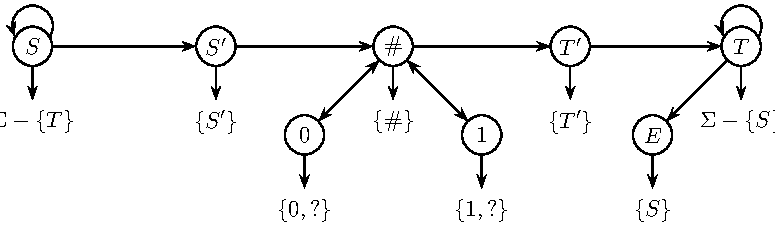
\includegraphics[scale=0.68]{../figures/jcss/cliquehmm.pdf}}
\caption[HMM for which footprint is NP-hard to optimize]{\label{fig:footprint_hmm} The HMM from the proof of Theorem
  \ref{THEOREM::NPFOOT}. States are shown as circles; under each we
  list the set of symbols that the state emits with non-zero
  probability. Each of these symbols is emitted with probability
  $1/k$, where $k$ is the size of the set. The HMM always starts in
  state $S$. All outgoing transitions from a particular state have
  the same probability.}
\end{figure*}

%\begin{definition*}[The most probable footprint problem]
% Given an HMM $H$, sequence $X$
%of length $n$ and a number $p\in [0,1]$, decide if there exists a footprint $F$
%such that $\prob{f(\pi) = S, X\mid H}\geq p$
%\end{definition*}

\begin{proof}(Theorem \ref{THEOREM::NPFOOT})
We will prove NP-hardness by a reduction from the maximum clique problem
using the HMM in Figure 
\ref{fig:footprint_hmm} with eight states and
alphabet $\Sigma=\{S, S', T, T', \#, 0,$ $1, ?\}$. 

%Popis zakodovania grafu
Let $G=(V,E)$ be an undirected graph with $n$ vertices $V=\{1,2,\dots,n\}$. We
will encode it in a sequence $X$ over alphabet $\Sigma$ as follows.  For every
vertex $v\in V$, we create a block $X_v$ with $2n+3$ symbols:
$X_v=S'\#b_{v,1}\#b_{v,2}\#\dots\#b_{v,n}\#T'$, where $b_{i,j}=1$ if $i=j$,
$b_{i,j}=?$ if $(i,j)\in E$ and $b_{i,j}=0$ otherwise.  Sequence $X$ is a
concatenation of blocks for all vertices with additional first and last symbols:
$X=SX_1X_2\dots X_nT$.

All state paths that can generate $X$ have a similar structure. The first
symbol $S$ and several initial blocks are generated in state $S$, one
block, say $X_i$, is generated in states $S'$, $\#$, $0$, $1$, and
$T'$ and the rest of the sequence, including the final symbol $T$, is
generated in state $T$. We will say that a state path with this
structure \emph{covers} the block $X_i$.  Note that state $E$ is never used in
generating $X$, its role is to ensure that the probability of
self-transition is the same in states $S$ and $T$.
All state paths that can generate $X$ have the same
probability $q = \Pr(\pi,X\mid H) = 2^{-2n^2-2n}3^{-n-1}7^{-2n^2-n+1}$.

%celkovo 2n^2+3n+2 symbolov
%1/2 zacni v S
%kazdy symbol v S a T ma 1/7 emisiu a 1/2 tranziciu do dalsieho
% tych symbolov je 2n^2+n-1
%prechody z S' a T', 0, 1 su 1, tych je n+2
%prechody z # so 1/3, tych je n+1
%emisia v S' a T' a # je 1, tych je n+3
%emisia v 0 a 1 je 1/2, tych je n
%
%spolu teda 1/2^{1 + 2n^2+n-1 + n} * 1/3^{n+1} * 1/7^{2n^2+n-1} 


We say that a state path $\pi$ is a \emph{run} of footprint $F$, if
$\pi$ can generate $X$, and $f(\pi)=F$.
Every footprint that can generate $X$ has the following structure:
$F=SS'\#c_1\#c_2\#\dots\#$ $c_n\#T'T$, where $c_i\in\{0,1\}$. 
The probability of footprint $F$ is $qk$, where $k$ is the number of its runs.
Also note that every run of $F$ covers a different $X_i$, because once $X_i$
and $F$ are fixed, the whole path is uniquely determined. 

We will now prove that the graph $G$ has a clique of size at least $k$
if and only if there is a footprint for sequence $X$ with
probability at least $qk$.  First, let $R$ be a clique in $G$ of size
at least $k>0$.  Consider the footprint
$F=SS'\#c_1\#c_2\#\dots\#c_n\#T'T$ where $c_i=1$ if $i\in R$ and $c_i=0$
otherwise. For any $i\in R$, there is a run $\pi_i$ of $F$ that covers
$X_i$. This run will use state 1 for generating each $b_{i,j}$ such
that $j\in R$ and thus both $b_{i,j}\in \{?,1\}$ and $c_j=1$.  For
$j\notin R$ we have $b_{i,j}=0$ and $c_j=0$, thus they will use state
0 in $\pi$. Since there is a different run for every $i\in R$, footprint 
$F$ has at least $k$ runs.



Conversely, let $F$ be a footprint with probability at least $qk>0$
and thus with at least $k$ runs. We will construct a clique of size at
least $k$ as follows. Let $R$ be the set of all vertices $i$ such that
$F$ has a run that covers $X_i$. Clearly the size of $R$ is at least
$k$.  Since $F$ has non-zero probability, it has the form
$SS'\#c_1\#c_2\dots\#c_n\#T'T$ for $c_i\in \{0,1\}$. For all $i\in R$,
$c_i=1$ because the $i$-th block has $b_{i,i}=1$. Therefore for all
$i,j\in R$, we have $b_{i,j}\in \{1,?\}$, which means that $(i,j)\in
E$ or $i=j$. This implies that $R$ is indeed a clique.

To summarize, given graph $G$ and threshold $k$, we can compute in
polynomial time sequence $X$ and threshold $qk$ such that $G$ has a
clique of size at least $k$ if and only if sequence $X$ has a
footprint with probability at least $qk$. This completes our reduction.

The problem is in NP (even if HMM is not fixed, but given on input),
because given an HMM $H$, sequence $X$ and a footprint $F$, we can
compute the probability $\Pr(f(\pi)=F,X\mid H,|X|)$ in polynomial time
by a dynamic programming algorithm which considers all prefixes of
$X$ and all prefixes of $F$. If probability $p$ and parameters of HMMs
are given as rational numbers, we can compute all quantities without
rounding in polynomial number of bits. \qed
\end{proof}

\subsection{The Most Probable Set Problem}\label{SECTION:NPSETALT}
In this section, we show an alternative proof of NP-hardness of the most
probable set problem. We show how to modify the proof of theorem \ref{THEOREM::NPFOOT}
to obtain a proof of theorem \ref{THEOREM::NPSET}.

%\begin{definition*}[The most probable set problem] Given an HMM $H$, sequence $X$ of
%length $n$ and a number $p\in [0,1]$, decide if there exists a set of states $S$
%such that $\prob{S(\pi) = S, X\mid H} \geq p$.
%\end{definition*}

\begin{figure*}
\centerline{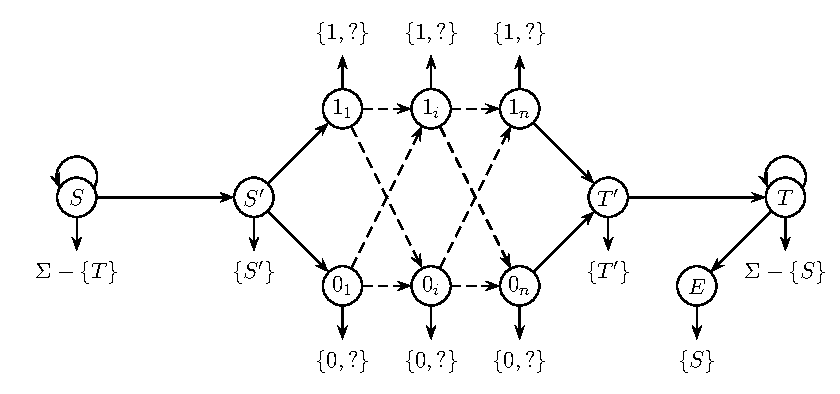
\includegraphics[scale=0.68]{../figures/jcss/expandedcliquehmm.pdf}}
\caption[HMM for which set is NP-hard to optimize]{The HMM from the proof of Theorem
  \ref{THEOREM::NPSET} for $n=3$. States are shown as circles; next to each we
  list the set of symbols that the state emits with non-zero
  probability. Each of these symbols is emitted with probability
  $1/k$, where $k$ is the size of the set. The HMM always starts in
  state $S$. All outgoing transitions from a particular state have
  the same probability.}\label{fig:set_hmm2}
\end{figure*}

\begin{proof}(Theorem \ref{THEOREM::NPSET})
Let $G=(V,E)$ be an undirected graph with $n$ vertices as in the proof of theorem
\ref{THEOREM::NPFOOT}. Note that $V = \{1, 2, \dots, n\}$. Graph $G$ will be encoded in
sequence $X$ as in the proof of theorem \ref{THEOREM::NPFOOT}, but without $\#$ symbols.
Let $X_i$ be the block that represents vertex $i$. Then $X=SX_1\dots X_nT$.

Instead of using one fixed HMM, we expand the middle part of the model so that it
generates blocks of length $n+2$ ($n$ vertices and $S', T'$ states). We remove
state $\#$ and expand states $0$ and $1$ into $n$ copies 
denoted $0_v$ and $1_v$ for $v \in V$.  Transitions are from $S'$ to $0_1$ and
$1_1$, from $0_n$ and $1_n$ to $T'$ and for all $i<n$ from $c_i$ to $d_{i+1}$
for $c,d\in \{0, 1\}$ as in figure  \ref{fig:set_hmm2}. 


State paths that generate $X$ have a similar structure as in the proof of theorem
\ref{THEOREM::NPFOOT}. State $S$ generate the first symbol $S$, and some initial blocks.
One block $X_i$ is generated by some of the states $S', T', 0_v, 1_v, v\in
V$.  Rest of the sequence is generated by the terminal state $T$.  Construction of
the HMM and sequence $X$ guarantees that for all $v\in V$ exactly one of $0_v, 1_v$
is in the state path. 
%Note that the set of states used in such a state
%path has exactly $n+4$ elements. 
We say that a state path with this structure
\emph{covers} block $X_i$. All state paths that can generate $X$ have the same
probability $q = \Pr(\pi, X\mid H) = 2^{-n^2-3n+1}6^{-n^2 - n}$.

We say that a state path $\pi$ is a \emph{run} of set $D$, if $\pi$ can generate
$X$ and $s(\pi) = D$. The probability of set $D$ is $qk$, where $k$ is the
number of runs of $D$. Every run of $D$ covers a different block, since once the
block is known, the path is uniquely determined.

We will now prove that the graph $G$ has a clique of size at least $k$ if and
only if there is a set of states for sequence $X$ with probability at least
$qk$.  First, let $R$ be a clique in $G$ of size at least $k>0$.  Consider the
set $D=\left\{S,S',{c_1},{c_2},\dots,{c_n},T',T\right\}$ where $c_i=1_i$ if
$i\in R$ and $c_i=0_i$ otherwise. For any $i\in R$, there is a run of
$D$ that covers $X_i$. This run will use state $1_j$ for generating each
$b_{i,j}$ such that $j\in R$ and thus both $b_{i,j}\in \{?,1\}$ and $c_j=1_j$.
For $j\notin R$ we have $b_{i,j}=0$ and $c_j=0_j$, thus the run will use state
$0_j$. Since there  is a different run for every $i\in R$, set $D$ has
at least $k$ runs.

Conversely, let $D$ be a set of states with probability at least $qk>0$
and thus with at least $k$ runs. We will construct a clique of size at least $k$
as follows. Let $R$ be the set of all vertices $i$ such that $D$ has a run that
covers $X_i$. Clearly the size of $R$ is at least $k$.  Since $D$ has non-zero
probability, it has the form $\left\{S,S',c_1,c_2,\dots,c_n,T',T\right\}$ for
$c_i\in \{0_i,1_i\}$. For all $i\in R$, $c_i=1_i$ because the $i$-th block has
$b_{i,i}=1$. Therefore for all $i,j\in R$, we have $b_{i,j}\in \{1,?\}$, which
means that $(i,j)\in E$ or $i=j$. This implies that $R$ is indeed a clique.

Given graph $G$ and threshold $k$, we can compute in
polynomial time sequence $X$ and threshold $qk$ such that $G$ has a
clique of size at least $k$ if and only if sequence $X$ has a
set of states with probability at least $qk$. This completes our reduction.\qed
\end{proof}
\subsection{The most probable restriction}
Finally, we show that the proof from the previous section is also proving NP-hardness of
the most probable restriction problem (Theorem \ref{THEOREM::NPREST}).

\begin{proof}(Theorem \ref{THEOREM::NPREST})
Consider the proof of Theorem \ref{THEOREM::NPSET} from Section
\ref{SECTION:NPSETALT}.
Any set for for sequence $X$ that have nonzero probability on sequences that
encodes graph with $n$ vertices have size $n + 4$. Therefore if we set $l = n +
4$ ($l$ is the restriction parameter), the proof of theorem
\ref{THEOREM::NPSET} is also a proof of this theorem.  \qed
\end{proof}
